\documentclass[../TDE4-E5.tex]{subfiles}%

\begin{document}
\section[s]"3"{Décrément logarithmique électrique}
\enonce{%
	On étudie la réponse $u(t)$ à un échelon de tension $e(t)$ tel que
	$ \left\{
		\begin{array}{rcl}
			e(t<0)    & = & 0 \\
			e(t\geq0) & = & E
		\end{array}
		\right.$
	dans le circuit ci-dessous.

	\begin{center}
		\sswitch{%
			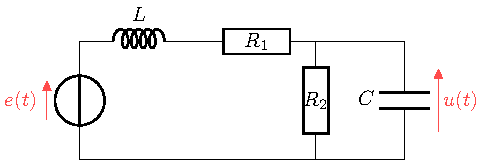
\includegraphics[width=.5\linewidth]{dec_log-plain}
		}{%
			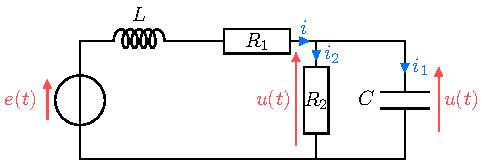
\includegraphics[width=.5\linewidth]{dec_log-intens}
		}%
	\end{center}
}%

\QR{%
	Déterminer la valeur $u_{\infty}$ vers laquelle tend $u(t)$ lorsque $t
		\longrightarrow \infty$.
}{%
	$R_2$ et $C$ sont en parallèle, donc $u(t)$ est à la fois la tension aux
	bornes de $C$ et de $R_2$. De plus, à $t \longrightarrow \infty$, la bobine
	se comporte comme un fil et le condensateur comme un interrupteur ouvert. Le
	circuit est donc équivalent à un diviseur de tension avec $R_1$ et $R_2$ en
	série alimentées par la tension $e(t)$, et on a donc
	\[ \boxed{u(\infty) = u_{\infty} = \frac{R_2}{R_1 + R_2}E}\]
}%

\QR{%
Montrer que $\DS \dv[2]{u}{t} + 2\lambda \dv{u}{t} +\w_0{}^2 u =
	\w_0{}^2u_{\infty}$. Exprimer $\lambda$ et $\w_0$ en fonction de $L$, $C$,
$R_1$ et $R_2$.
}{%
On applique les lois de \textsc{Kirchhoff}~:
\smallbreak
\begin{isd}
	Avec une loi des mailles et les relations courant-tension~:
	\[ u + L \dv{i}{t} + R_1i = E\]
	\tcblower
	Avec la loi des nœuds~:
	\begin{gather*}
		i = i_1 + i_2 = C \dv{u}{t} + \frac{u}{R_2}
	\end{gather*}
\end{isd}
En combinant~:
\begin{align*}
	u + L \dv{}{t} \left( C \dv{u}{t} + \frac{u}{R_2} \right) + R_1C
	\dv{u}{t} + R_1\frac{u}{R_2}                                          & = E
	\\\Lra
	u + LC \dv[2]{u}{t} + \frac{L}{R_2} \dv{u}{t} +
	R_1C \dv{u}{t} + \frac{R_1}{R_2}u                                     & = E
	\\\Lra
	LC \dv[2]{u}{t} + \left( \frac{L}{R_2} + R_1C
	\right)\dv{u}{t} + \left( \frac{R_1}{R_2} + \underset{
	\frac{R_2}{R_2}}{\cancel{1}} \right)u                                 & = E
	\\\Lra
	\dv[2]{u}{t} + \left( \frac{1}{R_2C} + \frac{R_1}{L}
	\right) \dv{u}{t} + \left( \frac{R_1 + R_2}{R_2} \right) \frac{u}{LC} & =
	\frac{E}{LC}
	\\\Lra
	\dv[2]{u}{t} + \left( \frac{1}{R_2C} + \frac{R_1}{L}
	\right) \dv{u}{t} +\left( \frac{R_1 + R_2}{R_2} \right)
	\frac{u}{LC}                                                          & = \left(\frac{R_1 + R_2}{R_2}\right)
	\frac{u_{\infty}}{LC}
	\\\Lra
	\Aboxed{\dv[2]{u}{t} + 2\lambda \dv{u}{t} + \w_0{}^2u                 & =
		\w_0{}^2u_\infty}
\end{align*}
\begin{gather*}
	\text{avec} \quad
	\boxed{
		\w_0 = \sqrt{\frac{1}{LC} \left( \frac{R_1 +
				R_2}{R_2} \right)}
	}
	\qet
	\boxed{
		\lambda = \frac{1}{2} \left(
		\frac{1}{R_2C} + \frac{R_1}{L} \right)
	}
\end{gather*}
}%

\QR{%
	On observe à l'oscilloscope la courbe $u(t)$ ci-contre, avec $\SI{1}{V/div}$
	de calibre vertical.
	\smallbreak
	\noindent
	\begin{minipage}{0.6\linewidth}
		\begin{enumerate}[label=\alph*)]
			\item Déterminer la valeur numérique de la pseudo-période $T$.
			\item Déterminer la valeur numérique du décrément logarithmique
			      \[\boxed{ \delta = \frac{1}{n} \ln \left( \frac{u(t) -
				      u_{\infty}}{u(t+nT)-u_{\infty}} \right)}\]
		\end{enumerate}
	\end{minipage}
	\begin{minipage}{0.4\linewidth}
		\centering
		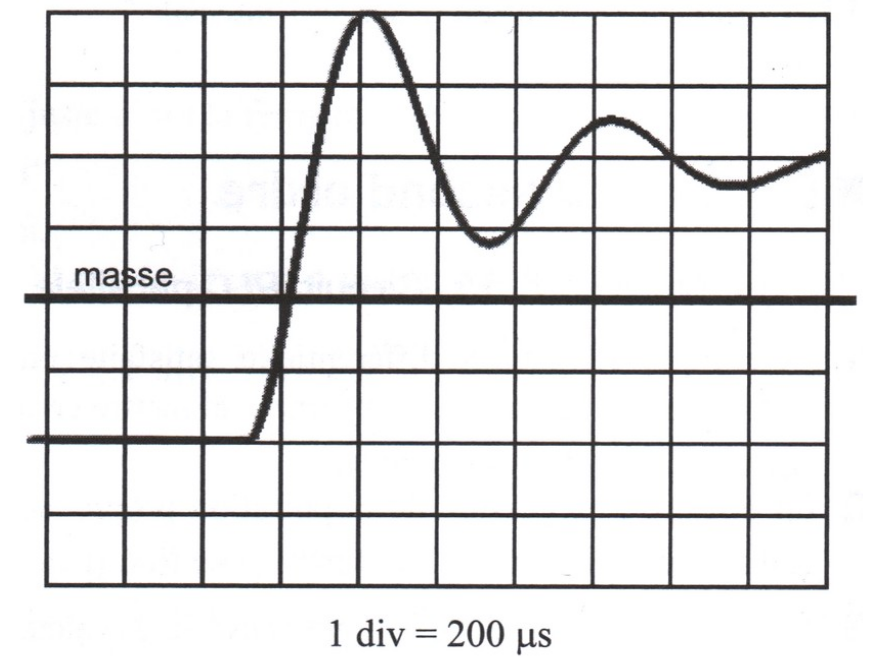
\includegraphics[width=\linewidth]{dec_log-courbe}
	\end{minipage}
}{%
	\begin{enumerate}[label=\alph*)]
		\item On a un régime pseudo-périodique, où on lit que \fbox{$T =
				      \SI{600}{\micro s}$}.
		\item On ne peut calculer $\delta$ qu'avec une pseudo-période ici. On
		      lit au premier pic à $t_1$ la valeur de la tension \textbf{par
			      rapport à la masse}~: $u(t_1) =
			      \SI{4}{V}$. Au second pic à $t_2 = t_1 + T$ on a~: $u(t_1 + T) =
			      \SI{2.5}{V}$. De plus, $u_\infty = \SI{2}{V}$. Ainsi,
		      \begin{equation*}
			      \boxed{\delta = \ln \left( \frac{4 - 2}{2.5-2} \right) = \ln(4)
				      = \num{1.39}}
		      \end{equation*}
	\end{enumerate}
}%

\QR{%
	Exprimer $u(t)$ en fonction de $u_{\infty}$, $\w_0$, $\lambda$ et $t$ (sans
	chercher à déterminer les constantes d'intégration).
}{%
	Pour la solution de l'équation homogène, on cherche les racines du polynôme
	caractéristique de discriminant $\Delta$~:
	\begin{gather*}
		r^2 + 2\lambda r + \w_0{}^2 = 0 \Rightarrow \Delta = 4(\lambda^2 - \w_0{}^2)
	\end{gather*}
	On sait que $\Delta < 0$ puisqu'on observe des oscillations amorties. On
	aura donc
	\begin{gather*}
		r_\pm = -\frac{\cancel{2}\lambda}{\cancel{2}} \pm \jj
		\frac{1}{\bcancel{2}}\sqrt{\bcancel{4}(\w_0{}^2 - \lambda^2)}
		\Leftrightarrow
		\boxed{r_\pm = -\lambda \pm \jj \w}
		\qavec
		\boxed{\w = \sqrt{\w_0{}^2 - \lambda^2}}
	\end{gather*}
	La solution particulière étant visiblement $u_\infty$, on aura la forme
	générale
	\begin{equation*}
		\boxed{u(t) = \exr^{-\lambda t} \left( A\cos\wt + B\sin\wt \right) +
			u_\infty}
	\end{equation*}
}%

\QR{Déterminer la relation entre $\delta$, $\lambda$ et $T$. En déduire la
	valeur numérique de $\lambda$.
}{
	Avec l'expression de $u(t)$, on peut développer le dénominateur de
	$\delta$~:
	\begin{gather*}
		u(t+nT) - u_\infty = \exr^{-\lambda nT}\times
		\underbrace{\exr^{-\lambda t}
			\left(
			A\underset{=\cos\wt}{\underline{\cos(\wt+n\wt)}} +
			B\underset{=\sin\wt}{\underline{\sin(\wt+n\wt)}}\right)
		}_{u(t) - u_\infty}
		\\
		\beforetext{Ainsi,}
		\frac{u(t) - u_\infty}{u(t+nT)-u_\infty} = \exr^{+\lambda nT}
		\Rightarrow
		\delta = \frac{1}{n} \ln (\exr^{\lambda nT})\\
		\Leftrightarrow \boxed{\delta = \lambda T \Leftrightarrow \lambda =
			\frac{\delta}{T}} \qavec \left\{
		\begin{array}{rcl}
			\delta & = & \num{1.39}         \\
			T      & = & \SI{600}{\micro s}
		\end{array}
		\right.\\
		\text{A.N.~:~}\xul{\lambda = \SI{2.32e3}{s^{-1}}}
	\end{gather*}
}

\QR{Sachant que $R_1 = \SI{200}{\ohm}$, $R_2 = \SI{5}{k\ohm}$ et $L =
		\SI{500}{mH}$, déterminer la valeur de $C$.
}{
	On sait que $\lambda$ s'exprime en fonction de $C$, on l'isole donc de son
	expression~:
	\begin{gather*}
		2\lambda = \frac{1}{R_2C} + \frac{R_1}{L}
		\Leftrightarrow
		R_2C = \frac{1}{2\lambda - \frac{R_1}{L}}\\
		\Leftrightarrow \boxed{C = \frac{1}{2R_2\lambda - \frac{R_1R_2}{L}}}
		\qavec
		\left\{
		\begin{array}{rcl}
			R_1     & = & \SI{200}{\ohm}      \\
			R_2     & = & \SI{5}{k\ohm}       \\
			L       & = & \SI{500}{mH}        \\
			\lambda & = & \SI{2.32e3}{s^{-1}}
		\end{array}
		\right.\\
		\text{A.N.~:~} \xul{C = \SI{76}{\micro F}}
	\end{gather*}
}
\siCorrige{
	\begin{tcb}[label=inte:declog](inte){À retenir}
		En régime pseudo-périodique, l'amortissement du signal est dû à
		l'exponentielle de la solution générale. En calculant le logarithme du
		rapport de la solution à un instant $t$ et de la solution à un instant
		$t+nT$ avec $T$ la période on calcule donc le facteur de l'exponentielle
		décroissante, ce qui permet de trouver les caractéristiques du circuit.
	\end{tcb}
}

\end{document}
